\documentclass[12pt,a4paper,oneside,openright,italian]{article}
\usepackage[italian]{babel}
\usepackage[latin1]{inputenc}
\usepackage{graphicx}
\usepackage{amsmath} 
\usepackage{amssymb}
\usepackage{verbatim}
\usepackage{longtable}
\usepackage{listings}


\newcommand{\degree}{\ensuremath{^\circ}}

\begin{document}

\title{Universit\`a degli Studi di Catania \\ Corso di Sensori e Trasduttori \\ Relazione sulle attivit\`a di laboratorio \\ A.A. 2008-2009}
\author{Giuseppe Monaco\footnote{A63/000134}, Natale Scigliano\footnote{178/401014}\\ Salvatore Maceo\footnote{615/000631}, Davide Marano\footnote{A63/000250}\\ Jacopo Cirrone\footnote{corso singolo}, Loris Fichera\footnote{A63/000232}}

\date{\today}  
\maketitle
\begin{abstract}
\`E stato condotto uno studio sperimentale il cui fine \`e stato la progettazione e sintetizzazione di un plantare posturale. A tale scopo \`e stato realizzato un plantare al cui interno \`e presente una matrice di sensori che rilevano la pressione esercitata sulla superficie del plantare stesso. 
I sensori utilizzati rientrano nella categoria dei sensori capacitivi, ovvero rilevano la pressione che viene esercitata fornendo in uscita una variazione di tensione, provocata dalla variazione della distanza tra le armature. Il sistema sviluppato \`e in grado di monitorare la pressione che il piede esercita su una superficie assumendo posture diverse o durante la normale deambulazione.

Buona parte del lavoro \`e stato effettuato dagli studenti Gerardo Trovato e Giovanni Trovato ed \`e descritto in \cite{trovato1}. Il contenuto di questa relazione riprende alcune delle tematiche trattate in \cite{trovato1} e lo integra con il contributo apportato dagli studenti del corso di Sensori e Trasduttori riguardo il circuito di generazione della portante e il sistema di interfacciamento sensore-PC.
\end{abstract}

\section{Introduzione ai sensori polimerici}
Il lavoro descritto in \cite{trovato1} ha anche lo scopo di studiare il comportamento di un particolare materiale polimerico: l'Elastosil LR 3162 A, B, un prodotto commerciale della Wacker. Il prodotto presenta buone propriet\`a sia meccaniche sia elettriche e una veloce vulcanizzazione. \`E composto da due componenti A e B che sono miscelati in rapporto di 1:1 per circa 30 min con aggiunta di trifluorocloroetilene. Alla fine di questa fase il composto acquisisce una consistenza gommosa. La deposizione del prodotto avviene tramite una maschera. In seguito, il prototipo realizzato viene messo in forno ad una temperatura di circa 120 \degree C per circa 30 min in modo tale che si abbia l'evaporazione  del trifluorocloroetilene, la vulcanizzazione e la conseguente adesione del materiale al supporto. Sperimentalmente si \`e osservata una vulcanizzazione, non aggiungendo del trifluorocloroetilene anche a temperatura ambiente o semplicemente sotto l'irraggiamento di una lampada ad incandescenza.
\begin{figure}[!hbp]
  \centering
  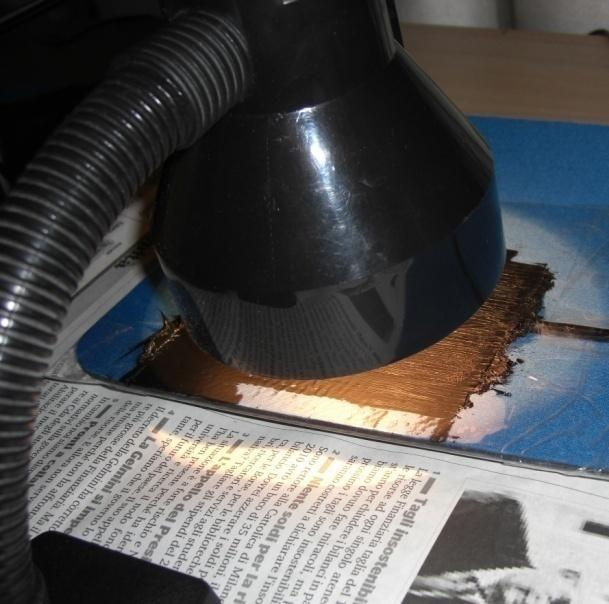
\includegraphics[width=250pt]{immagini/lampada.jpg}
  \caption{Vulcanizzazione dell'Elastosil}
  \label{elastosil}
\end{figure}

Il vantaggio di utilizzare tale tecnologia polimerica \`e quello di poter realizzare delle superfici conduttive con le propriet\`a meccaniche dei materiali gommosi, come ad esempio l'alta flessibilit\`a e l'elasticit\`a. Prima del processo di vulcanizzazione, infatti, il materiale \`e spalmabile su superfici di diversa natura, senza l'uso di particolari strumenti.

\section{Il sistema}

Di seguito viene riportato uno schema a blocchi dell'intero sistema realizzato.
\begin{figure}[!hbp]
  \centering
  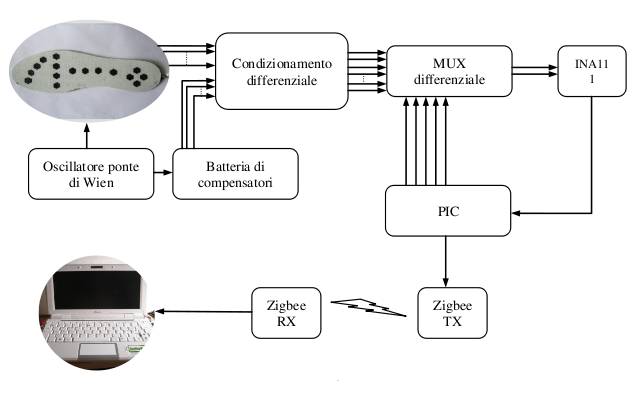
\includegraphics[width=350pt]{immagini/schema.png}
  \caption{Schema a blocchi del sistema}
  \label{condizionamento}
\end{figure}

\subsection{Il sensore}
La capacit\`a di un condensatore a facce piane parallele \`e inversamente proporzionale alla distanza delle armature. Interponendo come dielettrico uno strato di silicone o di altro materiale con una costante elastica opportuna si ha, a fronte di una pressione, una deformazione che produce una diminuzione della distanza. Essendo gli altri parametri costanti risulta quindi:
\begin{equation}
 C = f(d)
\end{equation}
Si crea in questo modo un trasduttore in grado di convertire una variazione di pressione in una variazione di distanza e, conseguentemente di capacit\`a, la quale, tramite un opportuno circuito di condizionamento, viene facilmente convertita in variazione di tensione. 

La matrice dei sensori \`e stata realizzata creando 16 isole di materiale polimerico, di forma esagonale, di lato 1 cm su un comune plantare, che creano cosi l'armatura mobile dei 16 condensatori. 

\begin{figure}[!hbp]
  \centering
  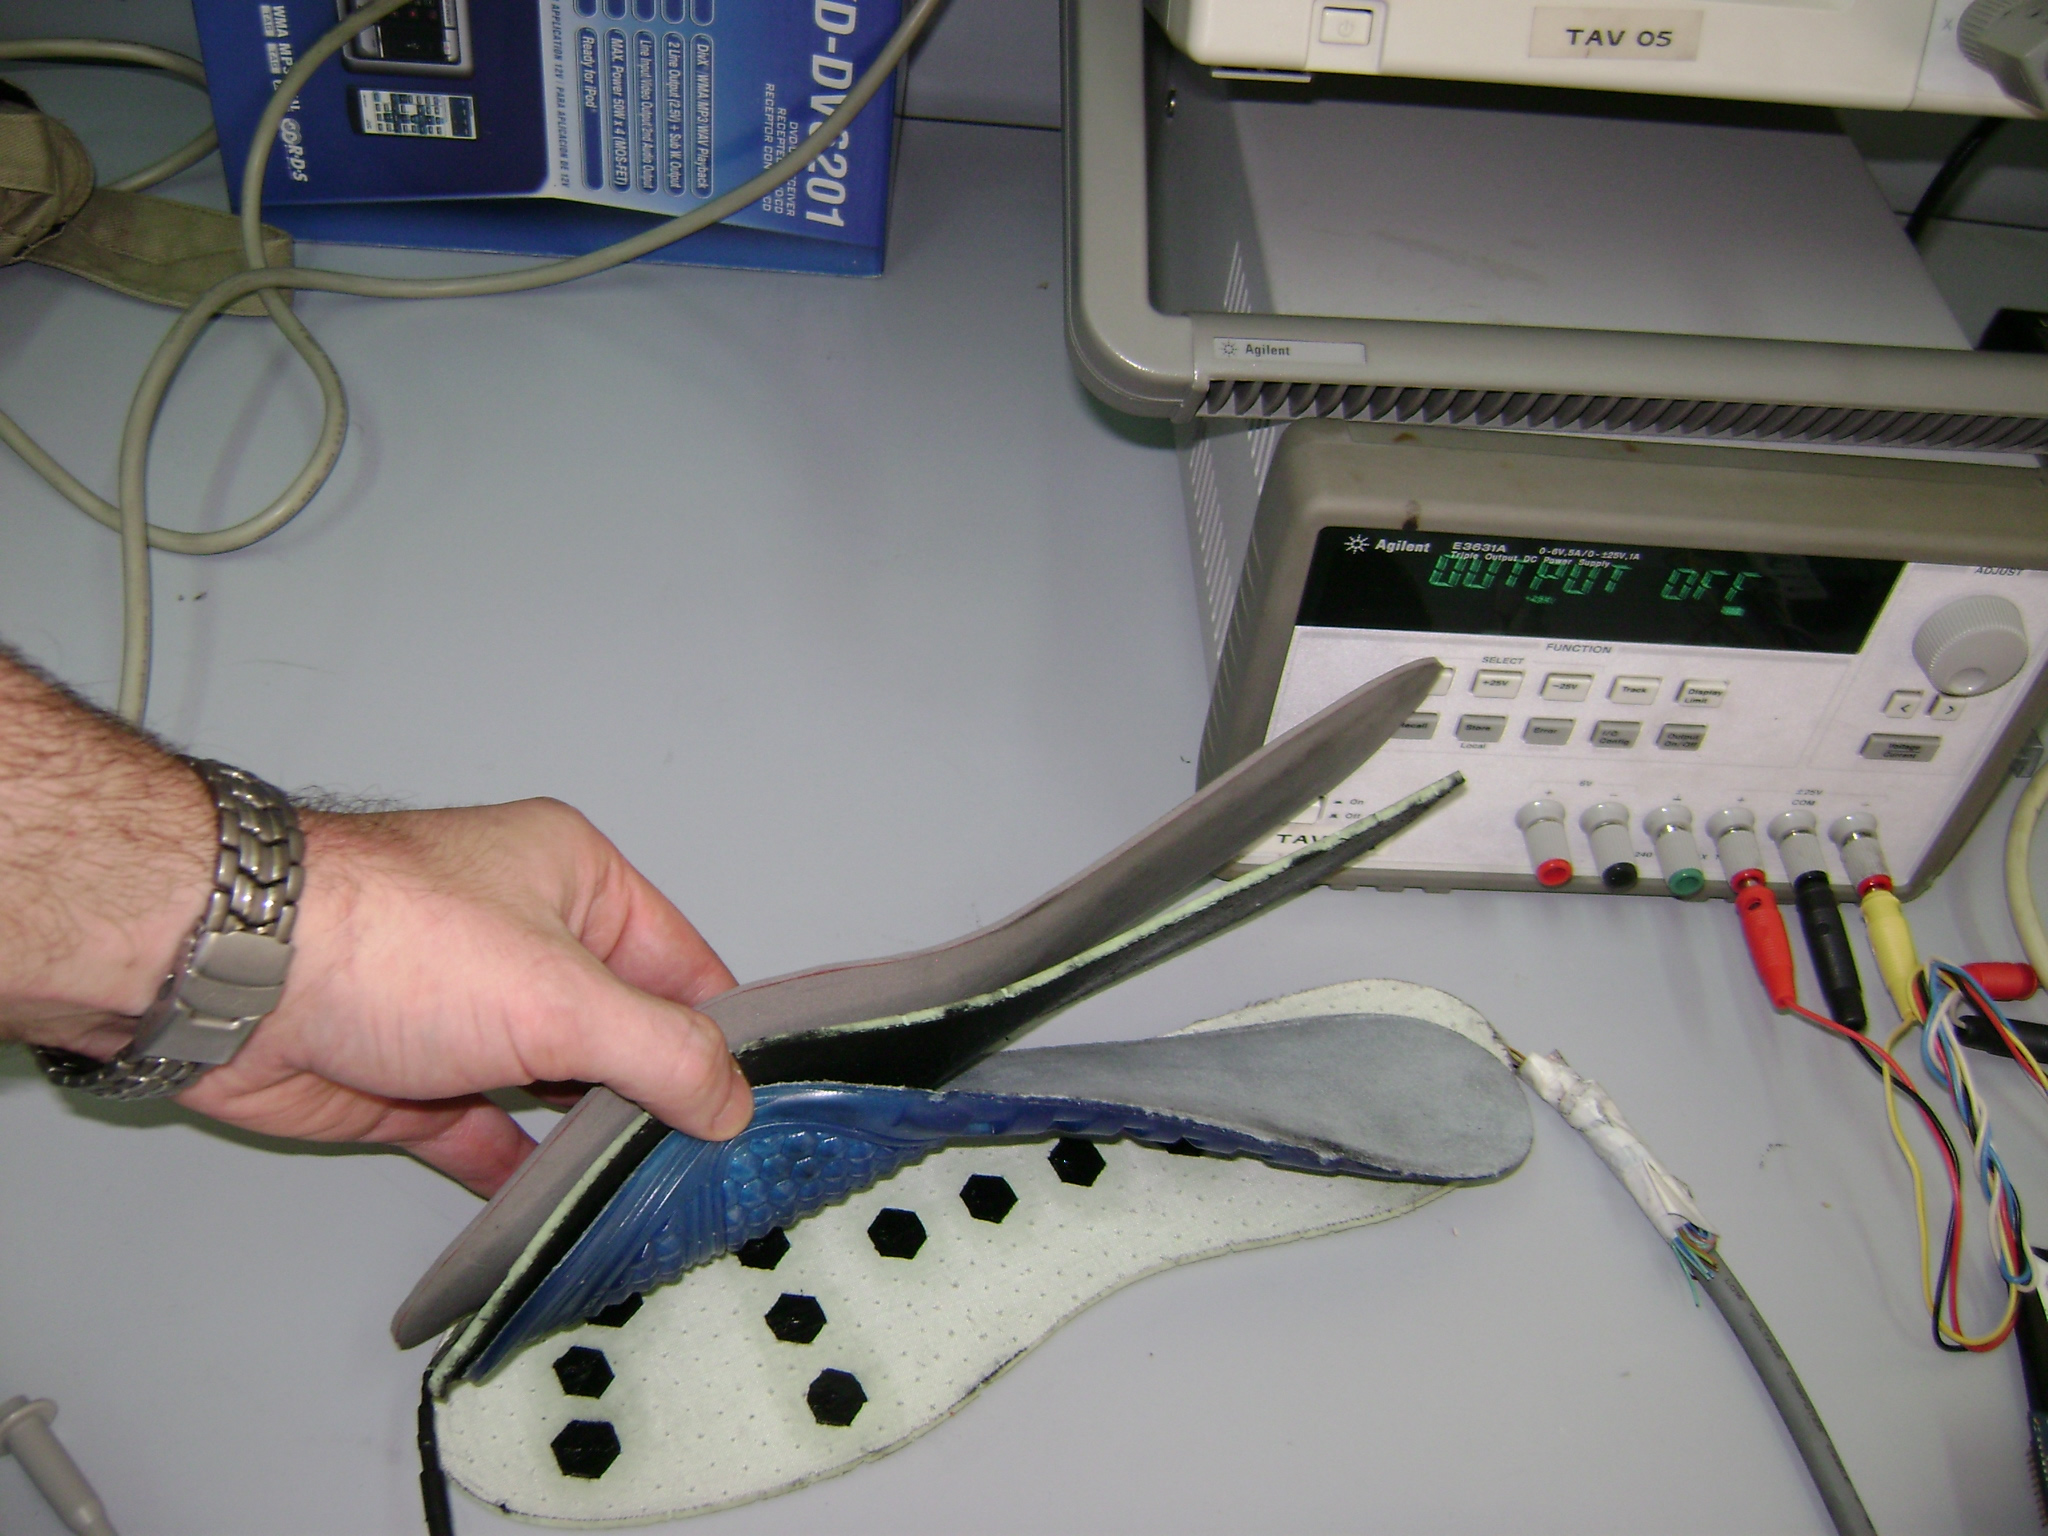
\includegraphics[width=320pt]{immagini/dsc00675.jpg}
  \caption{Il sensore plantare}
  \label{sensore}
\end{figure}

L'altra armatura \`e stata realizzata ricoprendo l'intera superficie di un ulteriore plantare, realizzando cosi un'unica armatura comune. Questa scelta progettuale ha lo scopo di eliminare eventuali disallineamenti tra le due armature che costituisco il singolo condensatore, che avrebbero determinato una variazione ulteriore e non voluta della superficie utile nel caso di slittamento tra i 2 plantari. 
\newline
Per aumentare l'elasticit\`a del wafer cos\`i ottenuto si \`e interposto tra i due plantari un ulteriore plantare di materiale elastico garantendo cosi un rapido ritorno in seguito alle sollecitazioni meccaniche. I collegamenti elettrici sono stati realizzati semplicemente immergendo le estremit\`a di un cavo a 16 fili nelle singole isole ancora non vulcanizzate,  stessa cosa \`e stata fatta sull'armatura comune con l'unica differenza che il cavo usato presentava un unico conduttore schermato, con il quale si fornisce alla matrice di sensori il segnale sinusoidale generato dall'oscillatore locale.
\begin{figure}[!hbp]
  \centering
  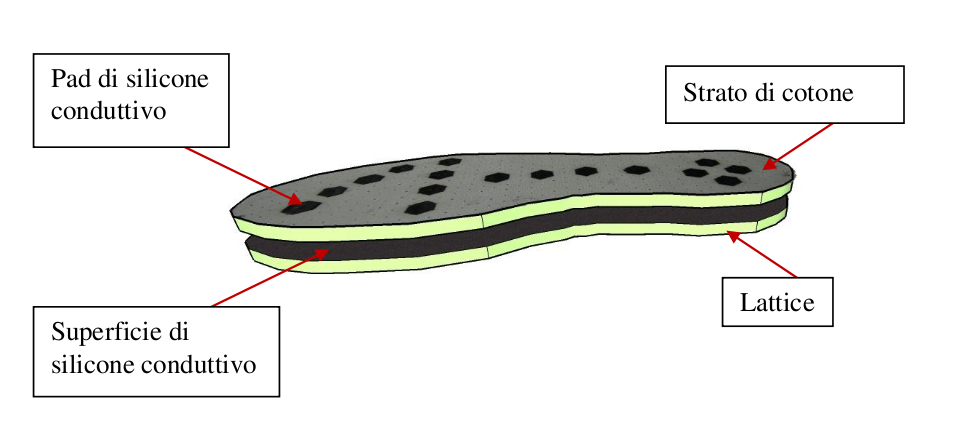
\includegraphics[width=350pt]{immagini/plantare.png}
  \caption{Modello 3D del plantare}
  \label{plantare3d}
\end{figure}

\subsection{Generatore di portante}
Si ha la necessit\`a di fornire al sensore un segnale sinusoidale con valore medio nullo avente frequenza di circa 100 kHz con un'ampiezza di circa 3 Vpp. Tale segnale viene generato tramite un circuito oscillante a ponte di Wien. La configurazione utilizzata \`e una di quelle consigliate dal produttore degli Amplificatori Operazionali. In particolare prevede l'utilizzo di due amplificatori operazionali, anzich\'e uno, e di alcuni filtri RC che elevano la qualit\`a del segnale di uscita. Lo schema del circuito \`e rappresentato in figura \ref{portante}.
%\newpage
\begin{figure}[!hbp]
  \centering
  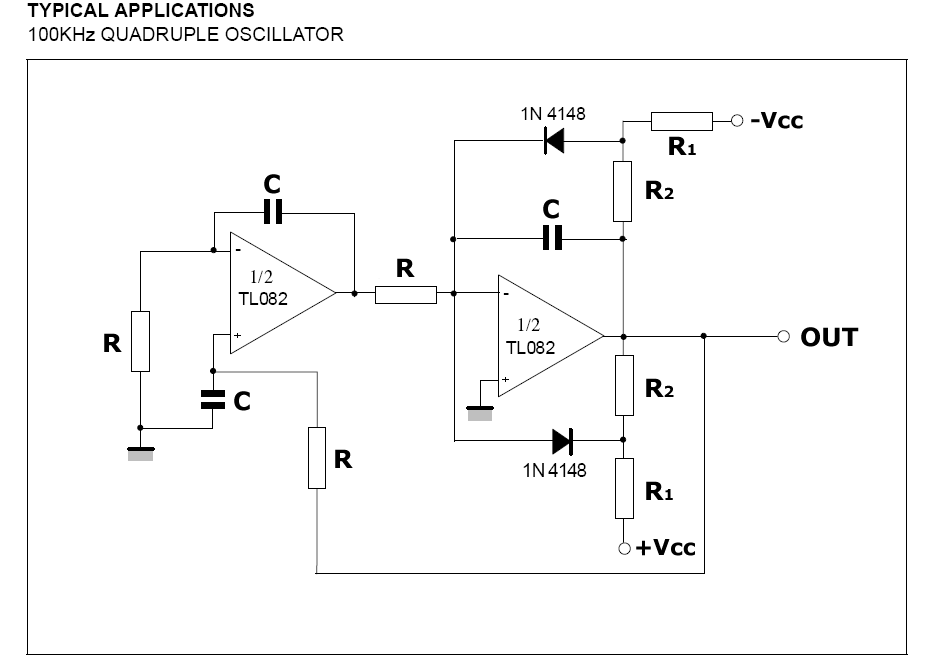
\includegraphics[width=350pt]{immagini/portante.png}
  \caption{Circuito di generazione della portante}
  \label{portante}
\end{figure}

Il circuito genera una sinusoide la cui frequenza viene determinata dalla seguente relazione:
\begin{equation} 
f = {1 \over 2\pi*RC}
\end{equation}
tramite la quale si sono opportunamente dimensionati i valori di R e C, per ottenere la frequenza desiderata. Gli input progettuali non richiedono valori di frequenza variabili, di conseguenza non si \`e ritenuto opportuno usare componenti variabili, in modo da minimizzare la superficie occupata dal circuito e anche il costo della componentistica.
Il \emph{ponte di Wien} \`e un circuito a retroazione positiva che amplifica e filtra il rumore bianco insito nel circuito stesso. Tale amplificazione deve essere variata dinamicamente per evitare la saturazione in uscita. Tale compito \`e svolto dalla coppia di diodi \emph{1N 4148} usati come resistori variabili. Nello stato di OFF offrono una resistenza elevata e conseguentemente guadagno elevato. Appena entrano in conduzione la resistenza diminuisce fino a raggiungere il guadagno unitario.
Per garantire il valore medio nullo del segnale di uscita \`e stata realizzata una rete di resistenze in uscita. Dai test effettuati sul circuito si \`e appurato che il segnale sinusoidale ha una frequenza di 98.8 kHz e una ampiezza di 1.2 Vpp. All'oscilloscopio la forma d'onda non presenta deformazioni evidenti sia a vuoto che con il carico. Visti i risultati ottenuti dai test e la minima superficie occupata dal circuito, non \`e stato ritenuto opportuno studiare eventuali migliorie.

\subsection{Circuito di condizionamento}
Inizialmente, al fine di rilevare la variazione di capacit\`a, si \`e deciso di adoperare, come circuito di condizionamento, un charge amplifier che rileva l'iniezione di carica.
\begin{figure}[!hbp]
  \centering
  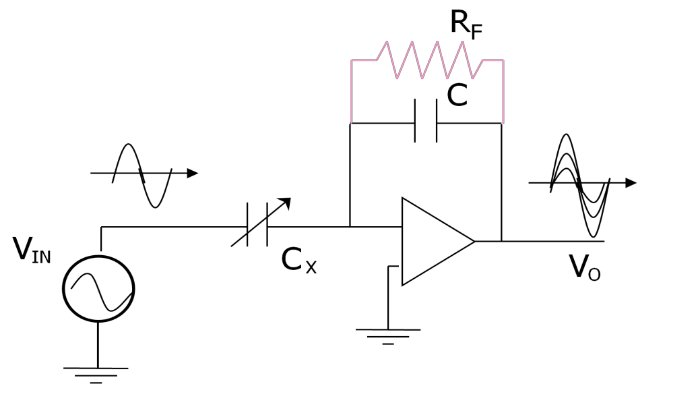
\includegraphics[width=350pt]{immagini/chargeamplifier.jpg}
  \caption{Circuito Charge Amplifier con resistenza di retroazione}
  \label{chargeampl}
\end{figure}
\newline
Trascurando la resistenza $R_f$ di retroazione e ricordando che la tensione ai capi del condensatore $C_x$ \`e data da:
\begin{equation}
V_{in} = {1 \over C_x} \int \! i_x \, dt
\end{equation}
e che,
\begin{equation}
V_o = - { 1\over C} \int \! i \, dt
\end{equation}
e che, per la legge di Kirchoff,
\begin{equation}
i_x = i
\end{equation}
si ha che:
\begin{equation}
V_o = -{C_x \over C} V_{in}
\end{equation}
Ricordando che $C_x$ \`e esprimibile come 
\begin{equation}
C_x = \varepsilon {A \over x}
\end{equation}
otteniamo una relazione diretta tra la tensione di uscita e la distanza x tra le armature, mantenendo, ovviamente, costanti gli altri parametri.  
\newline
Per evitare che la corrente di bias vada a caricare la capacit\`a, \`e necessario fornire una via alternativa per la corrente. Aggiungiamo quindi una resistenza di retroazione ottenendo in questo modo un circuito dal comportamento \emph{passa-banda}. Questo approccio fornisce gi\`a delle buone prestazioni, tuttavia per aumentare la sensibilit\`a del circuito di condizionamento si \`e deciso di progettare un circuito differenziale. Lo schema circuitale \`e presentato in figura \ref{condizionamento}. Il segnale sinusoidale fornito dall'oscillatore viene applicato ai due rami di amplificazione, il cui guadagno dipende dalle capacit\`a $C_{sensore}$, che corrisponde alla capacit\`a incognita del sensore, e $C_{I0}$, capacit\`a nota. I segnali in uscita a questi stadi d'amplificazione vengono opportunamente filtrati e mandati in ingresso ad un amplificatore di misura INA111. In definitiva, il segnale in uscita a tale circuito sar\`a un valore di tensione continua proporzionale al valore della capacit\`a incognita, che potr\`a essere quindi calcolato in maniera molto semplice:
\begin{equation}
V_{0-} = - {C_{xSensore} \over C} V_{in}
\end{equation}

\begin{equation}
V_{0+} = - {C_{I0} \over C} V_{in}
\end{equation}

\begin{equation}
V_{outINA} = 1 + {50 k\Omega \over R_G}
\end{equation}

dove $R_G$ \`e la resistenza di guadagno dell'INA111.

Come si \`e detto, il circuito in questione \`e stato dimensionato opportunamente per adattarlo ai valori di capacit\`a attesi. Si \`e agito, in particolare, sulle capacit\`a di retroazione $C_{I0}$, sulla sinusoide d'ingresso e sulle capacit\`a $C_{0A}$ e $C_{0B}$, mentre i valori degli altri componenti, elencati in tabella \ref{components}, sono rimasti invariati.

\begin{longtable}{|p{2,1cm}|p{2,1cm}|p{2,1cm}}
\endhead
\hline
Componente& Valore& Tolleranza\\
\hline
$R_{0A} R_{0B}$ &  1.5 M$\Omega$ & 5\%\\
\hline
$C_{F0A} C_{F0B}$ &  2.2 nF & 5\%\\
\hline
\caption{Componenti utilizzati}
\label{components}
\end{longtable}

Inizialmente, si \`e ipotizzato che la capacit\`a incognita $C_{sensore}$ fosse dell'ordine di qualche picofarad.



\begin{figure}[!hbp]
  \centering
  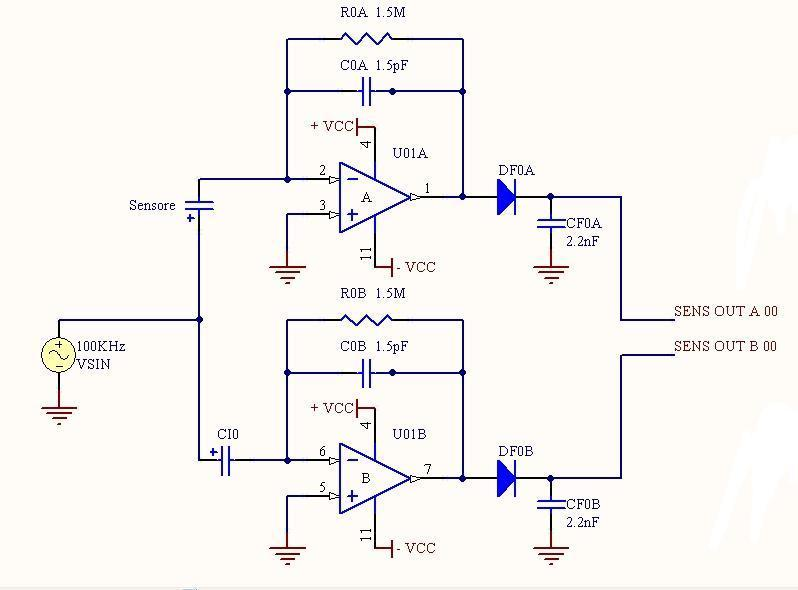
\includegraphics[width=230pt]{immagini/condizionamento.jpg}
  \caption{Circuito di condizionamento differenziale}
  \label{condizionamento}
\end{figure}


\subsection{Multiplexing}
Al fine di monitorare quanti pi\`u sensori possibili \`e stato previsto una sezione di multiplexing ovviamente differenziale per interfacciarsi all'ingresso dell'INA111. A tale scopo sono stati utilizzati due MAX DG407 con 8 canali differenziali ciascuno. Come riportato in figura \ref{multiplexing}.

\begin{figure}[!hbp]
  \centering
  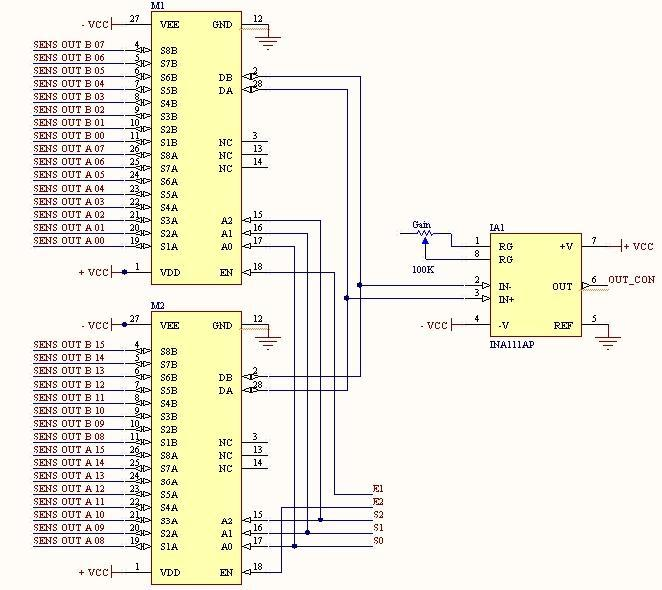
\includegraphics[width=310pt]{immagini/multiplexing.jpg}
  \caption{Circuito di multiplexing}
  \label{multiplexing}
\end{figure}

Si pu\`o notare che entrambe le uscite dei MUX sono collegate all'INA111 quindi per un corretto funzionamento \`e necessario controllare che, mentre un MUX sta lavorando, l'altro deve essere disabilitato, in modo che le uscite si portino ad uno stato di alta impedenza. Si noti che i due enable ed i tre selettori vengono pilotati direttamente dal microcontrollore PIC.


\newpage
\subsection{Acquisizione dei segnali}
La conversione A/D dei segnali provenienti dai singoli sensori avviene sfruttando il modulo di conversione A/D fornito da un microcontrollore \emph{PIC 18F2431}\cite{18f2431}.
\begin{figure}[!hbp]
  \centering
  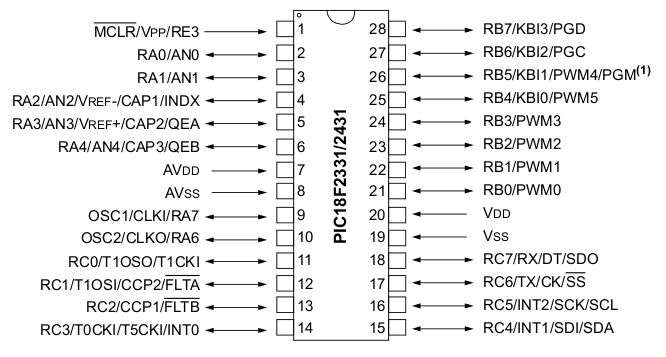
\includegraphics[width=390pt]{immagini/18f2431.png}
  \caption{Microcontrollore PIC 18F2431}
  \label{18f2431}
\end{figure}

Il microcontrollore \`e stato programmato per convertire ciclicamente i segnali provenienti dai singoli sensori in segnali digitali. La scelta del segnale da convertire \`e effettuata mediante il pilotaggio dei due multiplexer. Quattro pin di \emph{PORTB} sono utilizzati a questo scopo: uno per la selezione del MUX, gli altri tre per il pilotaggio del MUX scelto. La procedura principale del microcontrollore \`e, dunque, cos\`i strutturata:

\lstset{basicstyle=\scriptsize, numbers=left, breaklines=true, morecomment=[l]{//}}
\begin{lstlisting}[caption={Procedura principale del microcontrollore}, label={code:struct},frame=trBL]
void main()
{
	unsigned multiSelector = 0;
	...
	for(;;)
	{
		PORTB = multiSelector;
		...
		multiSelector++;
		multiSelector = multiSelector % 16;
	}	
}
\end{lstlisting}

Il modulo A/D del \emph{PIC 18F2431} permette di convertire segnali analogici compresi tra 0 e 5 volts in segnali digitali a 10 bit. Vi sono cinque canali disponibil, tuttavia, per la nostra applicazione, basta un solo canale. I registri del modulo sono stati settati come descritto da listato \ref{code:conf}.

\lstset{basicstyle=\scriptsize, numbers=left, breaklines=true, morecomment=[l]{//}}
\begin{lstlisting}[caption={Configurazione dei registri del modulo A/D}, label={code:conf},frame=trBL]
ADCON0 = 0b00000100; //Single channel, Single Shot

ADCON1 = 0b11001101; //Vref+ = Ext, Vref- = Ext, 

ADCON2 = 0b11111101; //Meno significativi, 64 Tad, Fosc/16

ADCON3 = 0b00000000; //No trigger

ANSEL0 = 0b00001110; //AN3, AN2, AN1 input analogici.

ADCON0 = ADCON0 | 1; //Attiva il convertitore
\end{lstlisting}

Menzione particolare merita il registro \emph{ADCON2}: il bit pi\`u alto serve a indicare la posizione del bit pi\`u significativo del segnale converito (nel nostro caso, questi sar\`a il bit pi\`u a destra), i successivi quattro bit indicano la durata dell'acquisizione (nel nostro caso, avendo settato tutti i bit a uno, questi sar\`a pari a 64 * Tad con Tad = 416 ns), gli ultimi tre bit settano la frequenza di lavoro del modulo A/D (la sequenza 101 identifica una frequenza pari a quella del clock del PIC diviso 16). Tali parametri sono stati calcolati empiricamente: se, da un lato, \`e necessario garantire una cert\`a rapidit\`a nel refresh del valore misurato dal singolo sensore, d'altra parte i segnali da campionare sono quasi statici. \`E stato sufficiente verificare che il pi\`u alto tempo di conversione garantiva ancora sufficiente rapidit\`a nel refresh dei valori misurati dai singoli sensori.

Al termine di ogni singola conversione, il microcontrollore scrive sulla propria uscita seriale una stringa codificata come segue:
\begin{equation}
  \$xy-abcd
\end{equation}
dove i bit xy identificano in maniera univoca un determinato sensore capacitivo (x identifica il MUX, y il canale attivo del MUX considerato), i bit abcd rappresentano il valore (compreso tra 0 e 1024) restituito dalla conversione A/D.

Dal punto di vista elettrico, il microcontrollore \`e stato alimentato con una tensione di 5 V sul piedino 20(Vdd), e massa sul piedino 19 (Vss). Sul piedino 1 \`e stato implementato il circuito di reset mostrato in figura \ref{reset}. \`E caratterizzato dalla presenza di una resistenza di carico, un diodo e un pulsante.

\begin{figure}[!hbp]
  \centering
  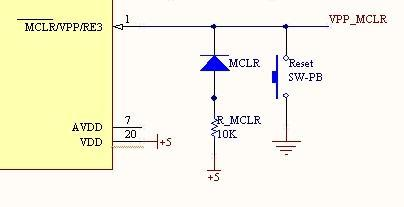
\includegraphics[width=250pt]{immagini/reset.jpg}
  \caption{Microcontrollore PIC 18F2431}
  \label{reset}
\end{figure}

L'ingresso al convertitore A/D \`e direttamente collegato con l'uscita dell'INA111 a cui \`e stato connesso in parallelo uno zener di limitazione a 5 Volt per evitare che un'eventuale sovratensione all'ingresso del convertitore A/D (piedino 3). I piedini 4 e 5 sono stati rispettivamente connessi a massa e a 5 V per impostare le soglie di riferimento. Il range di tensione utile in input, per una corretta conversione \`e quindi 0 V ÷ 5 V. Il circuito limitatore descritto \`e mostrato in figura \ref{limitatore}.

\begin{figure}[!hbp]
  \centering
  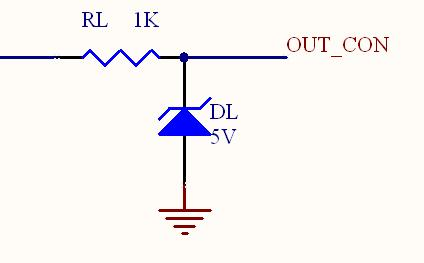
\includegraphics[width=250pt]{immagini/limitatore.jpg}
  \caption{Microcontrollore PIC 18F2431}
  \label{limitatore}
\end{figure}

\newpage
\subsection{Interfacciamento sensore-PC}
Il lavoro presentato in \cite{trovato1}, propone una semplice applicazione labview per la lettura e la rappresentazione grafica dei valori letti dai sensori capacitivi. L'interfacciamento tra microcontrollore e tale applicazione \` stato semplicemente realizzato a mezzo di un collegamento seriale RS-232. Volendo rendere il dispositivo di misura \emph{portatile}, sono stati utilizzati due dispositivi \emph{Xbee}\cite{xbee_datasheet} basati sullo standard \emph{IEEE 802.15.4}: uno di questi \`e stato collegato all'uscita seriale del microcontrollore, l'altro \`e stato collegato alla porta seriale del computer. Tra le varie modalit\`a di funzionamento supportate dai moduli \emph{Xbee} utilizzati vi \`e la \emph{transparent mode}: in questa modalit\`a, viene simulata la presenza di un bus seriale virtuale: il PIC e il computer comunicheranno attraverso questo bus, senza essere a conoscenza del fatto che il flusso dei dati viagger\`a su un canale wireless.

I moduli \emph{Xbee} vanno lavorano ad una tensione di 3.3 V. Al fine di interfacciarli correttamente con l'uscita seriale del microcontrollore e la porta seriale del computer, sono stati adottati i seguenti accorgimenti:
\begin{itemize}
\item pic $\rightarrow$ Xbee
  l'uscita seriale del PIC produce segnali di ampiezza pari a 5 Vpp. Per adattare il segnale alla logica del modulo Xbee \`e stato utilizzato un partitore di tensione, come mostrato in figura \ref{partitore}.

\item Xbee $\rightarrow$ PC
  l'uscita seriale del modulo Xbee produce segnali di ampiezza pari a 3.3 Vpp. Non \`e stato necessario adattare il livello del segnale in quanto le porte logiche CMOS associano tale valore al valore logico \emph{1}.
\end{itemize}

\begin{figure}[!hbp]
  \centering
  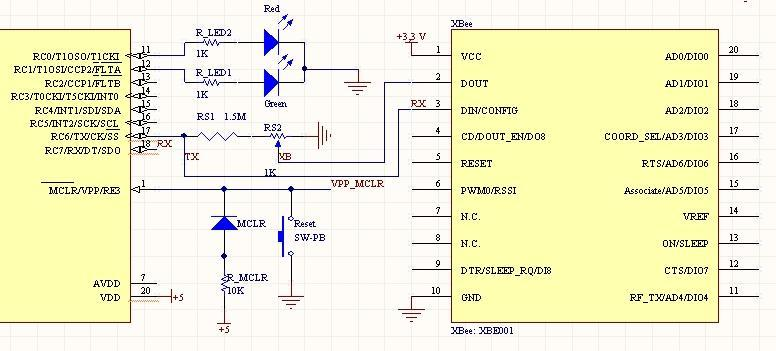
\includegraphics[width=280pt]{immagini/connessionepicxbee.jpg}
  \caption{M}
  \label{partitore}
\end{figure}

La struttura interna di un dispositivo Xbee \`e rappresentato in figura \ref{xbee}.
\begin{figure}[!hbp]
  \centering
  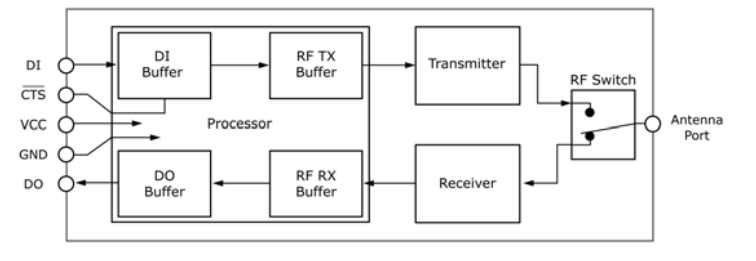
\includegraphics[width=390pt]{immagini/xbee_flow.png}
  \caption{Struttura interna di un modulo Xbee}
  \label{xbee}
\end{figure}

Sono presenti due buffer di memoria, uno per i dati in ingresso, l'altro per i dati ricevuti. Per poter comunicare correttamente, i dispositivi devono essere programmati in modo tale da decidere:
\begin{itemize}
\item il canale radio da utilizzare
\item il data rate del bus seriale virtuale
\item indirizzo del destinatario
\end{itemize}

Sfruttando la AT command mode, i moduli sono stati configurati con i seguenti parametri:

\begin{itemize}
\item data rate $\rightarrow$ 9600 b/s \\
  setta il data rate del bus seriale virtuale
\item channel $\rightarrow$ 1 \\
  setta il canale radio da utilizzare per la comunicazione
\item DH $\rightarrow$ * \\
  setta i bit pi\`u alti dell'indirizzo della destinazione
\item DL $\rightarrow$ * \\
  setta i bit pi\`u bassi dell'indirizzo della destinazione
\item RO $\rightarrow$ 0 \\
  setta il numero di caratteri di \emph{silenzio} da ascoltare prima dello svuotamento del buffer DI (settando RO = 0 ogni byte in ingresso alla porta seriale del dispositivo viene immediatamente spedito).
\end{itemize}

\subsection{Circuito di alimentazione}
Il circuito di alimentazione, in figura \ref{alimentazione} \`e utilizzato per ottenere 5 V e 3.3 V stabilizzati partendo dalla tensione di 9 V duale fornita da due batterie.

Come si evince dallo schema, non sono presenti n\'e il trasformatore n\'e il raddrizzatore con diodi a ponte in quanto la tensione fornita \`e gi\`a continua. Per stabilizzare la tensione si \`e utilizzato il componente LF50CP ed un LF33CP con package plastico in cui \`e previsto un foro al quale fissare una opportuna aletta di raffreddamento. I dispositivi hanno tre piedini di connessione che serviranno per la tensione d'ingresso, di uscita e la massa. I componenti hanno un limite di corrente massima di funzionamento di 1.0 A, valore abbondantemente compatibile con l'assorbimento del resto del circuito.

\begin{figure}[!hbp]
  \centering
  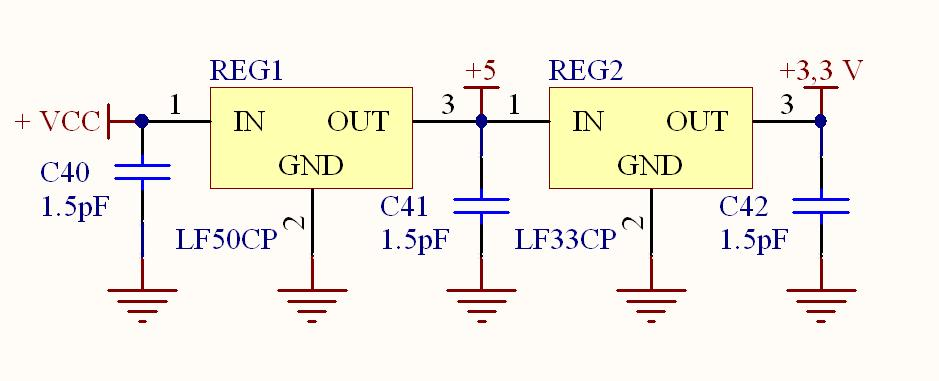
\includegraphics[width=220pt]{immagini/alimentazione.jpg}
  \caption{Circuito di alimentazione}
  \label{alimentazione}
\end{figure}

\subsection{Interfaccia LabView}
Per graficare i valori di tensione letti dal sensore si \`e scelto di implementare un'interfaccia grafica. Per tale interfaccia \`e stato scelto il linguaggio di programmazione LabVIEW.

\begin{figure}[!hbp]
  \centering
  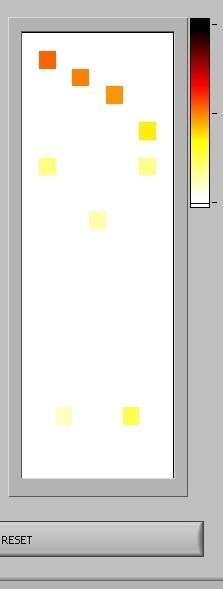
\includegraphics[width=220pt]{immagini/labview.jpg}
  \caption{Intefaccia LabVIEW}
  \label{alimentazione}
\end{figure}

Tale interfaccia presenta una rappresentazione 2D del plantare e, per ogni sensore, il valore letto viene rappresentato attraverso una scala di gradiente di colore: a colorazioni chiare corrispondono piccoli valori del misurando, a colorazioni pi\`u scure corrispondono valori del misurando maggiori.

Tale interfaccia \`e stata dotata di due particolari funzionalit\`a: una di \emph{reset} che sfrutta i valori memorizzati in condizione di carico minimo per fare in modo che i valore di uscita in tali condizioni siano nulli.
Al rilascio del pulsante di reset, i valori immagazzinati in condizioni di minimo carico, vengono sottratti al valore correntemente rilevato. In questo modo vengono rimossi via software gli inevitabili offset iniziali.

La seconda funzionalit\`apermette, attraverso la normalizzazione di avere degli output compresi tra 0 e 1. 
Alla pressione del tasto normalizza, infatti, alcune variabili locali memorizzano il contenuto dei valori rilevati dai sensori, mentre al rilascio , i dati acquisiti vengono divisi per il valore immagazzinato in memoria.

I dati ottenuti tramite il sistema di normalizzazione sono gi\`a pronti per essere stampati ma non risulta semplice associare il dato al sensore che lo ha prodotto. Per tale motivo le informazioni raccolte vengono inserite in un array tridimensionale in modo da mappare spazialmente la posizione originale. In questo risulta immediata l'associazione sensore - dato.
\newpage
\section{Caratterizzazione del sensore}
\subsection{Verifica della linerarit\`a}
In questo paragrafo verr\`a presentata la modalit\`a con la quale \`e stata verificata la linearit\`a del circuito di condizionamento. Per prima cosa \`e stata creata una ``batteria'' di capacit\`a campione con la quale si \`e studiato l'andamento d'uscita di ogni canale del circuito di condizionamento. Procedendo in modo sistematico si sono effettuate misure ripetute dell'uscita di ogni singolo canale al variare della capacit\`a campione ed il valore medio ottenuto \`e stato riportato in una tabella. Per motivi di semplificazione vengono riportati in figura \ref{taratura} i grafici dei canali 1, 2 e 9 del circuito di condizionamento.

\begin{figure}[!hbp]
  \centering
  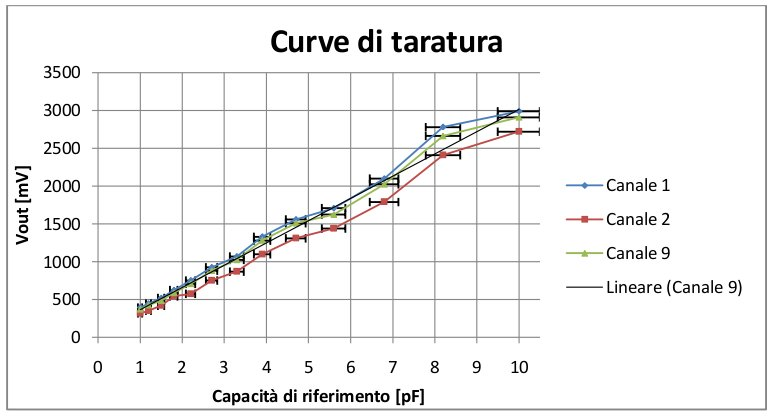
\includegraphics[width=220pt]{immagini/taratura.jpg}
  \caption{Curve di taratura}
  \label{taratura}
\end{figure}

Come si pu\`o notare dal grafico il circuito di condizionamento presenta una risposta sufficientemente lineare.

Il sistema utilizzato per definire la scala presenta numerose difficolt\`a. Prima di tutto, come descritto nel capitolo relativo, il circuito di condizionamento presenta una configurazione di tipo differenziale, per cui ogni canale possiede un offset differente in funzione del valore a cui \`e stata fissata la capacit\`a di riferimento. Un ulteriore problema si presenta nella sezione di amplificazione differenziale, dove il valore del resistore che determina il guadagno non pu\`o essere determinato a priori. Per ultimo, il sistema di acquisizione del segnale analogico tramite PIC prevede la conversione in livelli che vanno da 0 a 1024. Per ovviare a questi problemi si \`e proceduto per passi successivi, cercando di determinare la capacit\`a a vuoto e a carico massimo per poi risalire al valore di pressione esercitato sulla superficie del singolo sensore. Per prima cosa si \`e effettuata una campagna di acquisizioni ripetute a carico nullo. I valori cos\`i ottenuti sono strati traslati in basso di una quantit\`a pari al valore minimo, in modo da eliminare gli offset. In seguito \`e stata effettuata, varie volte, una campagna di acquisizioni durante differenti tipi di camminata e con vari tipi di carichi applicati al fine di identificare il valore massimo. Di tutti i valori massimi misurati \`e stata fatta una media, che \`e risultata essere 2,43 V. Utilizzando la curva di taratura precedentemente illustrata, si deduce che la capacit\`a misurata in caso di permettivit\`a massima \`e di circa 8 pF. Ricordando che la capacit\`a C nel caso specifico \`e data da:
\begin{equation}
C = {A \varepsilon \over d}
\end{equation}
si pu\`o ottenere il valore di d utilizzando la relazione inversa:
\begin{equation}
d = {A \varepsilon \over C}
\end{equation}
dove A \`e l'area della singola armatura esagonale di lato 1 cm ed \`e pari a 212 * 10$^{-6}$ m$^2$. Sostituendo i valori si ricava una distanza d = 0.77 mm. Dal valore ottenuto, conoscendo la costante elastica del silicone possiamo risalire alla pressione esercitata sul singolo sensore. Considerata la buona linearit\`a del circuito di condizionamento si pu\`o suddividere l'intervallo di valori acquisiti in parti uguali cos\`ida creare una scala lineare.

Al fine di testare il funzionamento del dispositivo sono stati effettuati test statici, dove il plantare acquisiva informazioni in condizioni di postura normale e di postura alterata, e test dinamici dove i dati venivano trasmessi in fase di deambulazione.

\subsection{Test statici}
Il dispositivo, opportunamente configurato tramite la regolazione delle capacit\`a di riferimento, permette di valutare i livelli di pressione in corrispondenza dei sensori. Si \`e cercato, quindi, di riprodurre alcune situazioni tipiche di errore di postura scorretta.

\begin{figure}[!hbp]
  \centering
  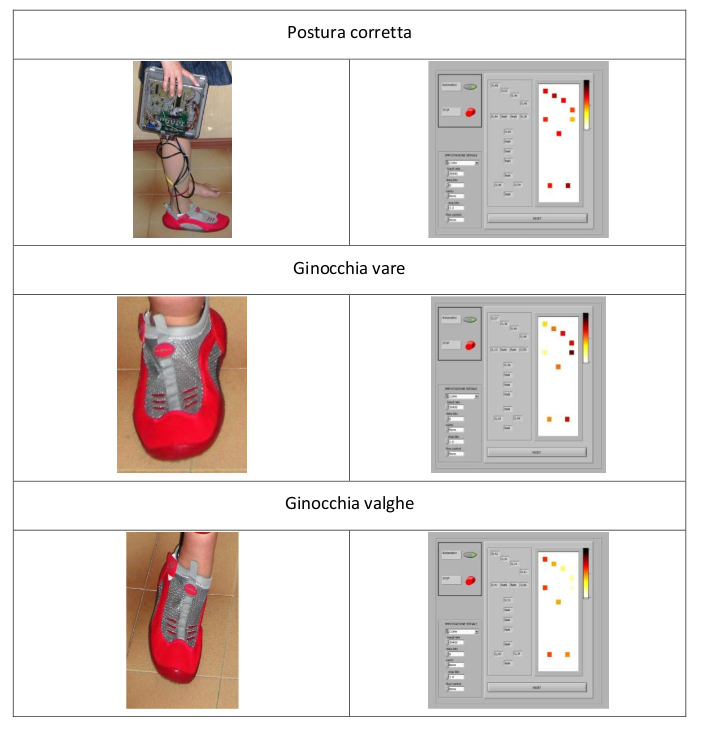
\includegraphics[width=370pt]{immagini/posture.png}
  \caption{Test statici}
  \label{static}
\end{figure}

Come si pu\`o notare dalla figura \ref{static}, nel caso della postura corretta i sensori centrali e quelli relativi al tallone presentano un maggiore livello, mentre, nel caso di valgismo rilevano una maggiore intensit\`a le aree interne della pianta. Analogamente nel caso di ginocchia vare si nota una visibile predominanza di intensit\`a nelle zone esterne.

\subsection{Test dinamici}
Come introdotto in precedenza per valutare la risposta del dispositivo sono stati effettuati alcuni test con un soggetto in fase di normale andatura. Contemporaneamente una sezione separata del programma in LabVIEW ha scritto su un file in formato .csv compatibile con i pi\`u comuni fogli di calcolo i valori relativi ad ogni sensore con frequenza costante di 25 campioni al secondo. I valori cos\`i ottenuti sono stati normalizzati e riportati in formato grafico in figura \ref{dynamic}.

\begin{figure}[!hbp]
  \centering
  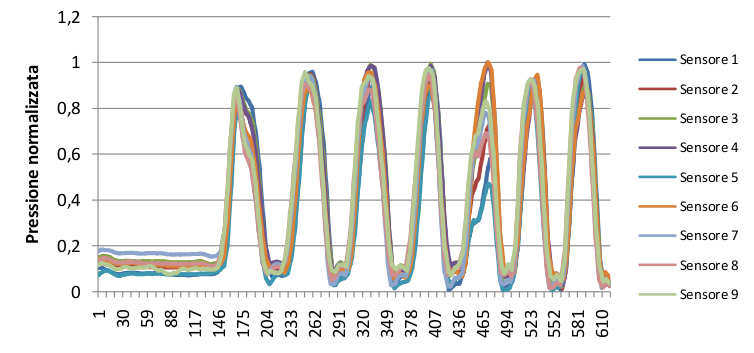
\includegraphics[width=330pt]{immagini/risposta.png}
  \caption{Test dinamici}
  \label{dynamic}
\end{figure}

Come si pu\`o notare da un rapido sguardo si pu\`o identificare un'area dove il soggetto mantiene il piede sollevato ed una porzione dove si nota un innalzamento a cadenza regolare del valore di pressione misurato. \`E possibile, inoltre, accorgersi di un'irregolarit\`a nel primo e nel quinto passo dovute ad una curvatura nell'incedere. Il grafico in figura \ref{singlestep} mostra invece il particolare di un passo regolare.

\begin{figure}[!hbp]
  \centering
  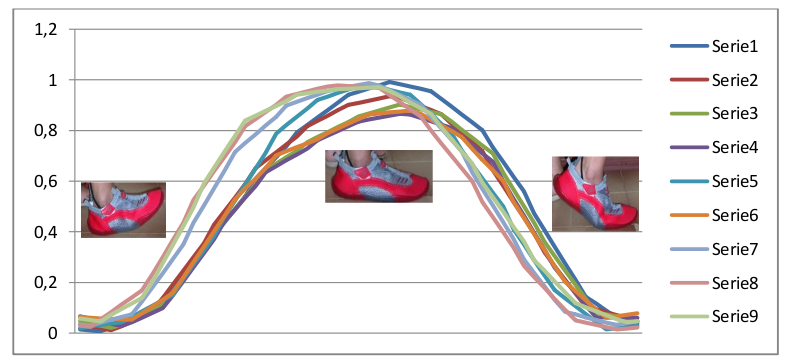
\includegraphics[width=330pt]{immagini/singlestep.png}
  \caption{Singolo passo}
  \label{singlestep}
\end{figure}

Risulta agevole notare che durante un normale passo i sensori relativi alla zona del tallone raggiungono il loro massimo prima ,il sensore centrale comincia a rilevare una variazione qualche decimo dopo ed infine i sensori posizionati nella parte superiore del piede commutano in istanti molto prossimi. Viceversa durante la fase di distacco del piede dal suolo i tempi di discesa del valore misurato risultano invertiti.

\newpage
\section{Sviluppi Futuri}
\subsection{Ottimizzazione del circuito di condizionamento}
Il circuito realizzato si presenta ancora sottoforma di prototipo su piastra millefori. Per misurare capacit\`a dell'ordine dei picofarad, come nel nostro caso, un circuito siffatto non risulta sufficientemente schermato dai rumori. Realizzando tutto il circuito su un'unica PCB si potrebbero ottenere sicuramente delle risposte pi\`u performanti. In primo luogo bisogna progettare dei buoni piani di massa, avendo cura, nel caso in cui si opti per una scheda a doppia faccia, di non far sovrapporre le piste per lunghi tratti rettilinei prima del circuito di condizionamento, evitando cos\`i fenomeni di interferenza. In secondo luogo si potrebbe anche pensare di separare la parte di circuito che processa dati analogici dai controlli che sono invece digitali. Un altro aspetto da tenere in considerazione sarebbe quello di utilizzare dei cavi schermati per diffondere il segnale dal sensore al resto del circuito. Per compensare lo sbilanciamento a monte dell'amplificatore differenziale (INA111) sono stati adoperati dei condensatori variabili. Questi per\`o risultano poco precisi e non mantengono il valore di capacit\`a costante per lunghi periodi.

\subsection{Aumento del numero di sensori}
Testato il funzionamento dei multiplexer differenziali, si potrebbe pensare di acquisire molti pi\`u canali realizzando un plantare con pi\`u sensori in modo da ottenere dei risultati pi\`u significativi e che meglio si prestano ad applicazioni biomediche.

\subsection{Altre modifiche}
Una specifica del progetto prevede la possibilit\`a di ottimizzare il circuito rendendolo il pi\`u piccolo possibile al fine di ovviare agli inconvenienti derivanti dall'uso di una postazione fissa. In questo modo sarebbe utile realizzare un sistema integrato, considerando cio\`e il circuito come parte  integrante della calzatura. Non si avrebbe cos\`i nessuna percezione  dell'utilizzo di un dispositivo di misurazione rendendo il test naturale e  non intralciando in alcun modo i movimenti durante la camminata o la  corsa. Per fare ci\`o si potrebbe pensare di realizzare una PCB compatta  impiegando solo componenti SMD che oltre a ridurre gli spazi, riducono le  capacit\`a parassite. Si potrebbe anche pensare di realizzare i sensori, non  pi\`u come tanti pads da un lato e una faccia comune a tutti dall'altro, bens\`i facendo incrociare delle fasce di silicone conduttivo poste in modo  ortogonale su due piani paralleli non coincidenti(vedi figura \ref{sviluppi}).  A questo punto, prima di acquisire, si dovrebbe attivare una riga ed una colonna per selezionare il capacitore corrispondente all'intersezione.  Sarebbe interessante prevedere un circuito di condizionamento con  multiplexer a monte limitando, in questo modo, ulteriormente la  dimensione del circuito. Un altro ovvio vantaggio che ne deriverebbe  sarebbe un numero minore di collegamenti verso il circuito di condizionamento a parit\`a di numero di sensori impiegati. Per ottenere  prestazioni migliori si potrebbe anche pensare di utilizzare dei PIC pi\`u  performanti onde ottenere velocit\`a di elaborazione e invio dei dati pi\`u rapido, con un ovvio aumento della velocit\`a di acquisizione. 

\begin{figure}[!hbp]
  \centering
  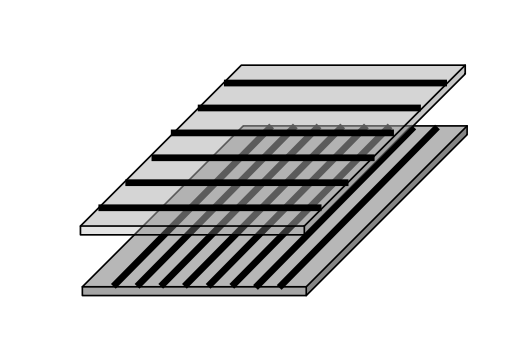
\includegraphics[width=330pt]{immagini/sviluppi.png}
  \caption{Sensore a griglia ortogonale}
  \label{sviluppi}
\end{figure}


\newpage
\section{Firmware del microcontrollore PIC}
\lstset{basicstyle=\scriptsize, numbers=left, breaklines=true, morecomment=[l]{//}}
\begin{lstlisting}[caption={Firmware}, label={code:pic},frame=trBL]
/*
	Silicon Sensor Firmware
*/

#include ".\common.h"
#include <delays.h>
#include <adc.h>
#include <usart.h>
#include <stdio.h>

#define RED_LED 	LATCbits.LATC0
#define GREEN_LED	LATCbits.LATC1

#define DEBUG_MODE

void printMessage (int value, int sensor_label);

void printMessage (int value, int sensor_label)
{
	/*
	string format is
	$XX-XXXX
    12345678 - eight byte needed
	*/

	char string_sensor_label[3];
	char string_value[5];
	char to_send[9];
	int i;

	//converting values into strings
	itoa(value,string_value);
	itoa(sensor_label,string_sensor_label);

	// string construction
	for (i = 0; i< 9; i++)
	{
		if (i==0)
			to_send[i] = '$';
		else if (i==3)
			to_send[i] = '-';
		else if ((i > 0) && (i < 3))
			to_send[i] = string_sensor_label[i-1];
		else if ((i > 3) && (i < 8))
			to_send[i] = string_value[i-4];
		else if (i == 8)
			to_send[i] = '\0';
	}
	
	// print the string
	printf("%s",to_send);
}
#endif

void Initialize (void)
{
	TRISB = 0xF0; //All Output Digital
	TRISC = 0x80; //100000000
	RED_LED = 0;
	GREEN_LED = 1;
	
	//Init ADC
	ADCON0 = 0b00000100; //Single channel, Single Shot
	ADCON1 = 0b11001101; //Vref+ = Ext, Vref- = Ext, 
	ADCON2 = 0b11111101; //Meno significativi, 64 Tad, Fosc/16
	ADCON3 = 0b00000000; //No trigger
	ADCHS = 0;			 //Setta i gruppi
	ANSEL0 = 0b00001110; //AN3, AN2, AN1 input analogici.
	TRISA = 0b00001110;
	ADCON0 = ADCON0 | 1; //Attiva il convertitore
	Delay10TCYx( 5 );		 
	
	//Init USART
	OpenUSART(USART_TX_INT_OFF  & USART_RX_INT_OFF  &
			  USART_ASYNCH_MODE & USART_EIGHT_BIT	&
			  USART_CONT_RX 	&
			  USART_BRGH_HIGH   , 32);

}

int getADC (void)
{
	int r;
	ADCON0 = ADCON0 | 2; //Avvia la conversione
	#ifdef DEBUG_MODE
	printf("\r\nConverting...\r\n");
	#endif

	while(ADCON0 & 0x02){}; //Aspetta la fine della conversione
	r = (ADRESH & 0x03) * 256 + (ADRESL);
	return r;
}

void main()
{
	unsigned char i, multiSelector = 0;
	
	Initialize();
	putrsUSART("Init...\r\n");
	while(1)
	{
		PORTB = multiSelector;
		Delay10KTCYx( 10 );
		result = getADC();
		RED_LED = 1 - RED_LED;
 		#ifdef DEBUG_MODE
 		//printf("ADC Converted!\r\n");
  		//printf("Valore %02d: %02d", multiSelector, result);
		#endif

		printMessage (int result, int multiSelector); //prints the message on the serial port
		
		multiSelector++;
		multiSelector = multiSelector % 16;
	}	
}
\end{lstlisting}

\newpage
\begin{thebibliography}{9}

\bibitem{trovato1} Giovanni Trovato e Gerardo Trovato, \emph{"Realizzazione di un plantare posturale a sensori capacitivi mediante silicone conduttivo"} \newline Universit\`a degli Studi di Catania 2009.

\bibitem{18f2431} Microchip PIC 18F2431, \emph{"PIC 18F2431 Data Sheet"} \newline http://ww1.microchip.com/downloads/en/DeviceDoc/39616C.pdf

\bibitem{xbee_datasheet} XBee \& XBee-PRO 802.15.4 OEM RF Modules, \emph{"XBee Modules Data Sheet"} \newline http://www.digi.com/register/index.jsp?mu=/pdf/ds\_xbeemultipointmodules.pdf
%% \bibitem{cellbreath} Bahl, P., Hajiaghayi, M.T., Jain, K., Mirrokni, S.V., Qiu, L., Saberi, A. (2007), \emph{Cell Breathing in Wireless LANs: Algorithms and Evaluation}, Mobile Computing, IEEE Transactions on , vol.6, no.2, pp.164-178, Feb. 2007

%% \bibitem{ns2} NS-2 Documentation, \emph{"The Network Simulator - ns-2: Documentation"} \newline http://www.isi.edu/nsnam/ns/ns-documentation.html
  
\end{thebibliography}
\end{document}
